\section{Results and Diagnostic Data}

A comprehensive diagnostic pipeline continuously broadcasts
internal controller states across a structured topic hierarchy
to objectively quantify algorithmic performance during active
testing. Data is presented separately for the two operating
modes: static home posture and dynamic trotting gait.

\subsection{Home Posture Stabilization}

During the static home posture, the quadruped maintains all four
limbs in ground contact while the PID controller actively
rejects base orientation disturbances.

Fig.~\ref{fig:home_results} presents the complete home mode
diagnostic dataset. The pitch axis measurement and error signals
(Fig.~\ref{fig:home_error}) show the base tilting under an
applied disturbance. The EMA filtered IMU measurement captures
the orientation deviation, while the deadband filtered error
signal demonstrates effective suppression of trivial oscillations
below the $\pm 0.02$~rad threshold. The gradual convergence
toward zero confirms the integral accumulator's correction
capability at steady state.

The corresponding PID correction output
(Fig.~\ref{fig:home_corr}) reveals that the saturated PID output
exhibits sharp transient spikes during rapid disturbance onset,
while the lowpass filtered output tracks the saturated signal
with significantly reduced high frequency content. The resulting
joint torque commands (Fig.~\ref{fig:home_joint}) settle from
initial transients into steady state values, confirming that the
multistage pipeline produces stable actuator commands suitable
for sustained static balancing.

\begin{figure}[htbp]
    \centering
    \begin{subfigure}[b]{0.44\columnwidth}
        \centering
        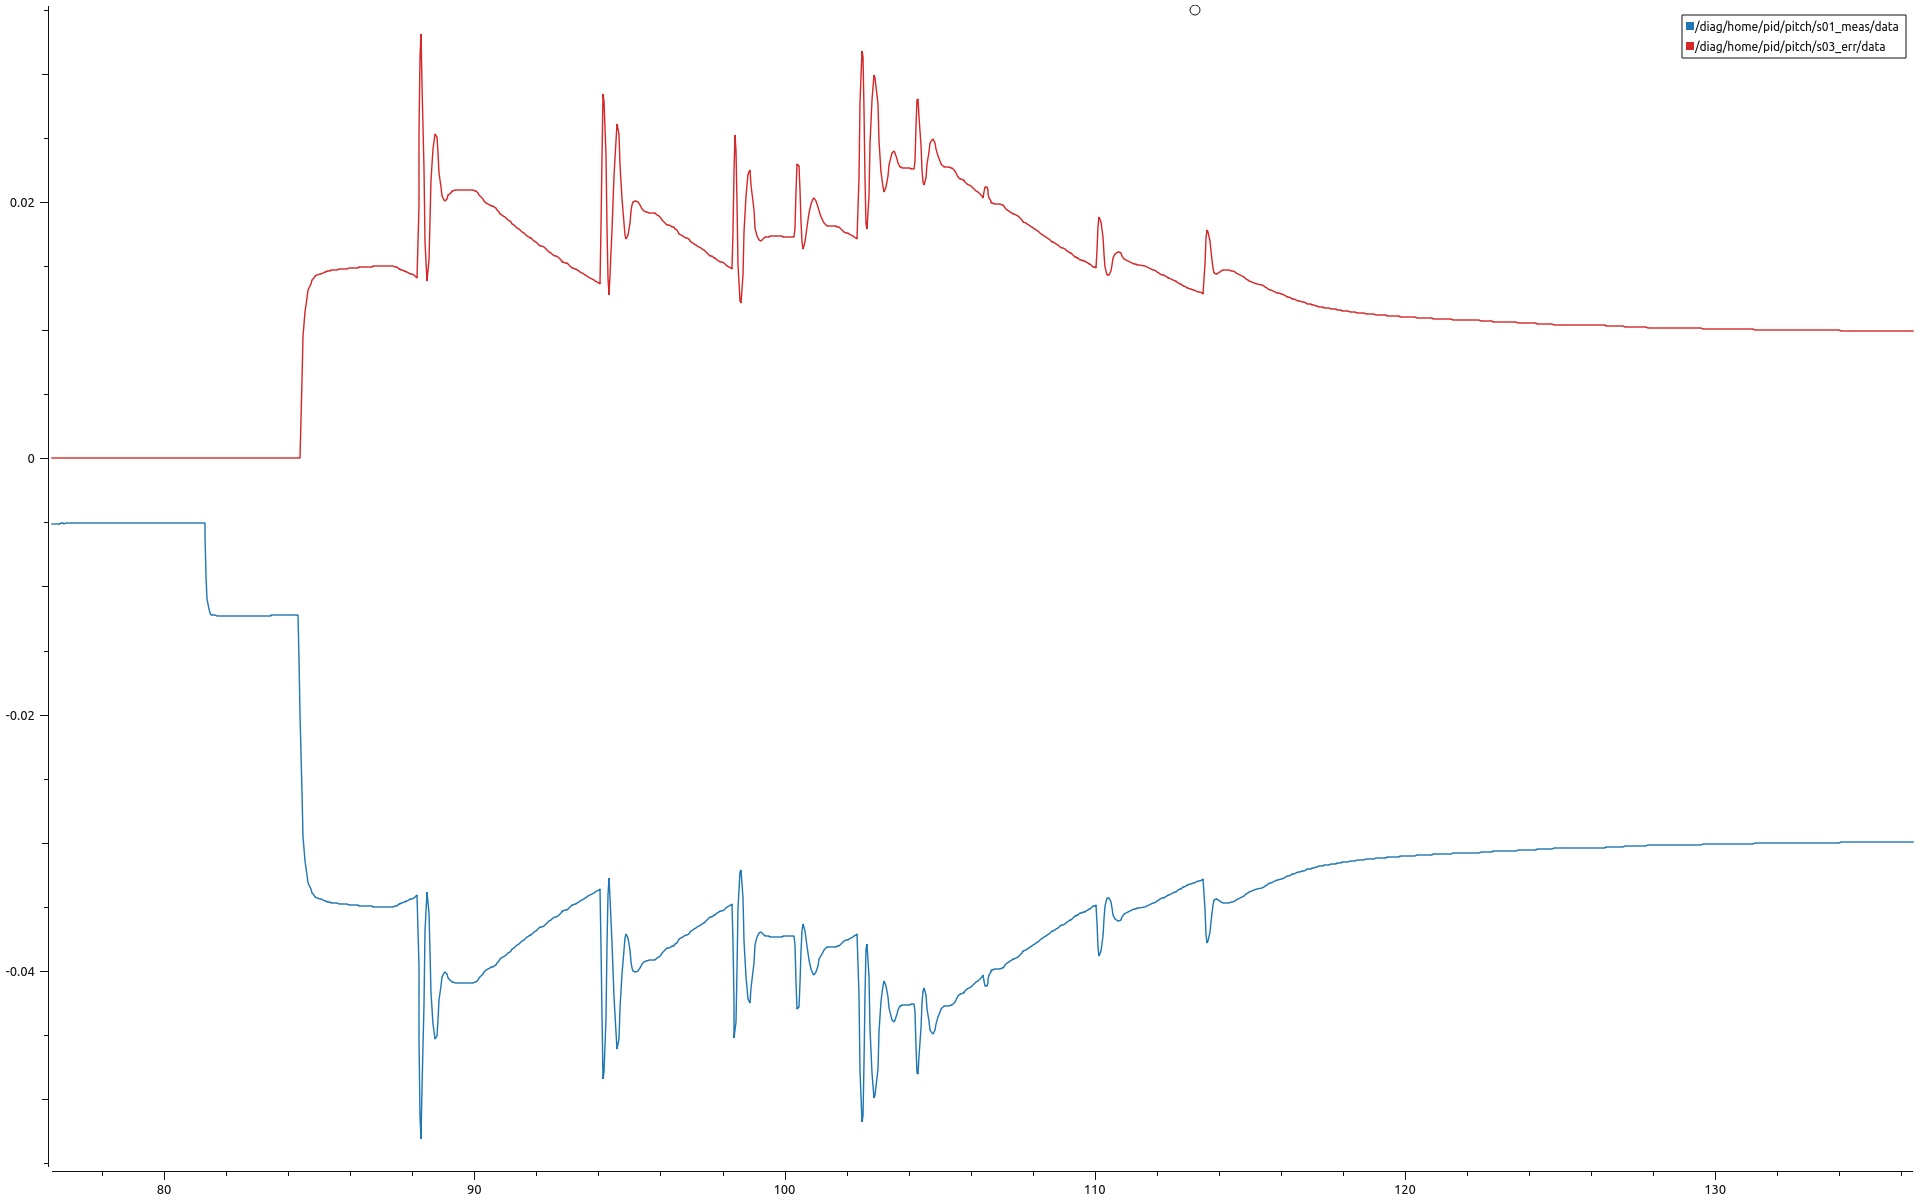
\includegraphics[width=\textwidth]{figures/imu_balance_homing_error.png}
        \caption{Pitch and error.}
        \label{fig:home_error}
    \end{subfigure}
    \hfill
    \begin{subfigure}[b]{0.44\columnwidth}
        \centering
        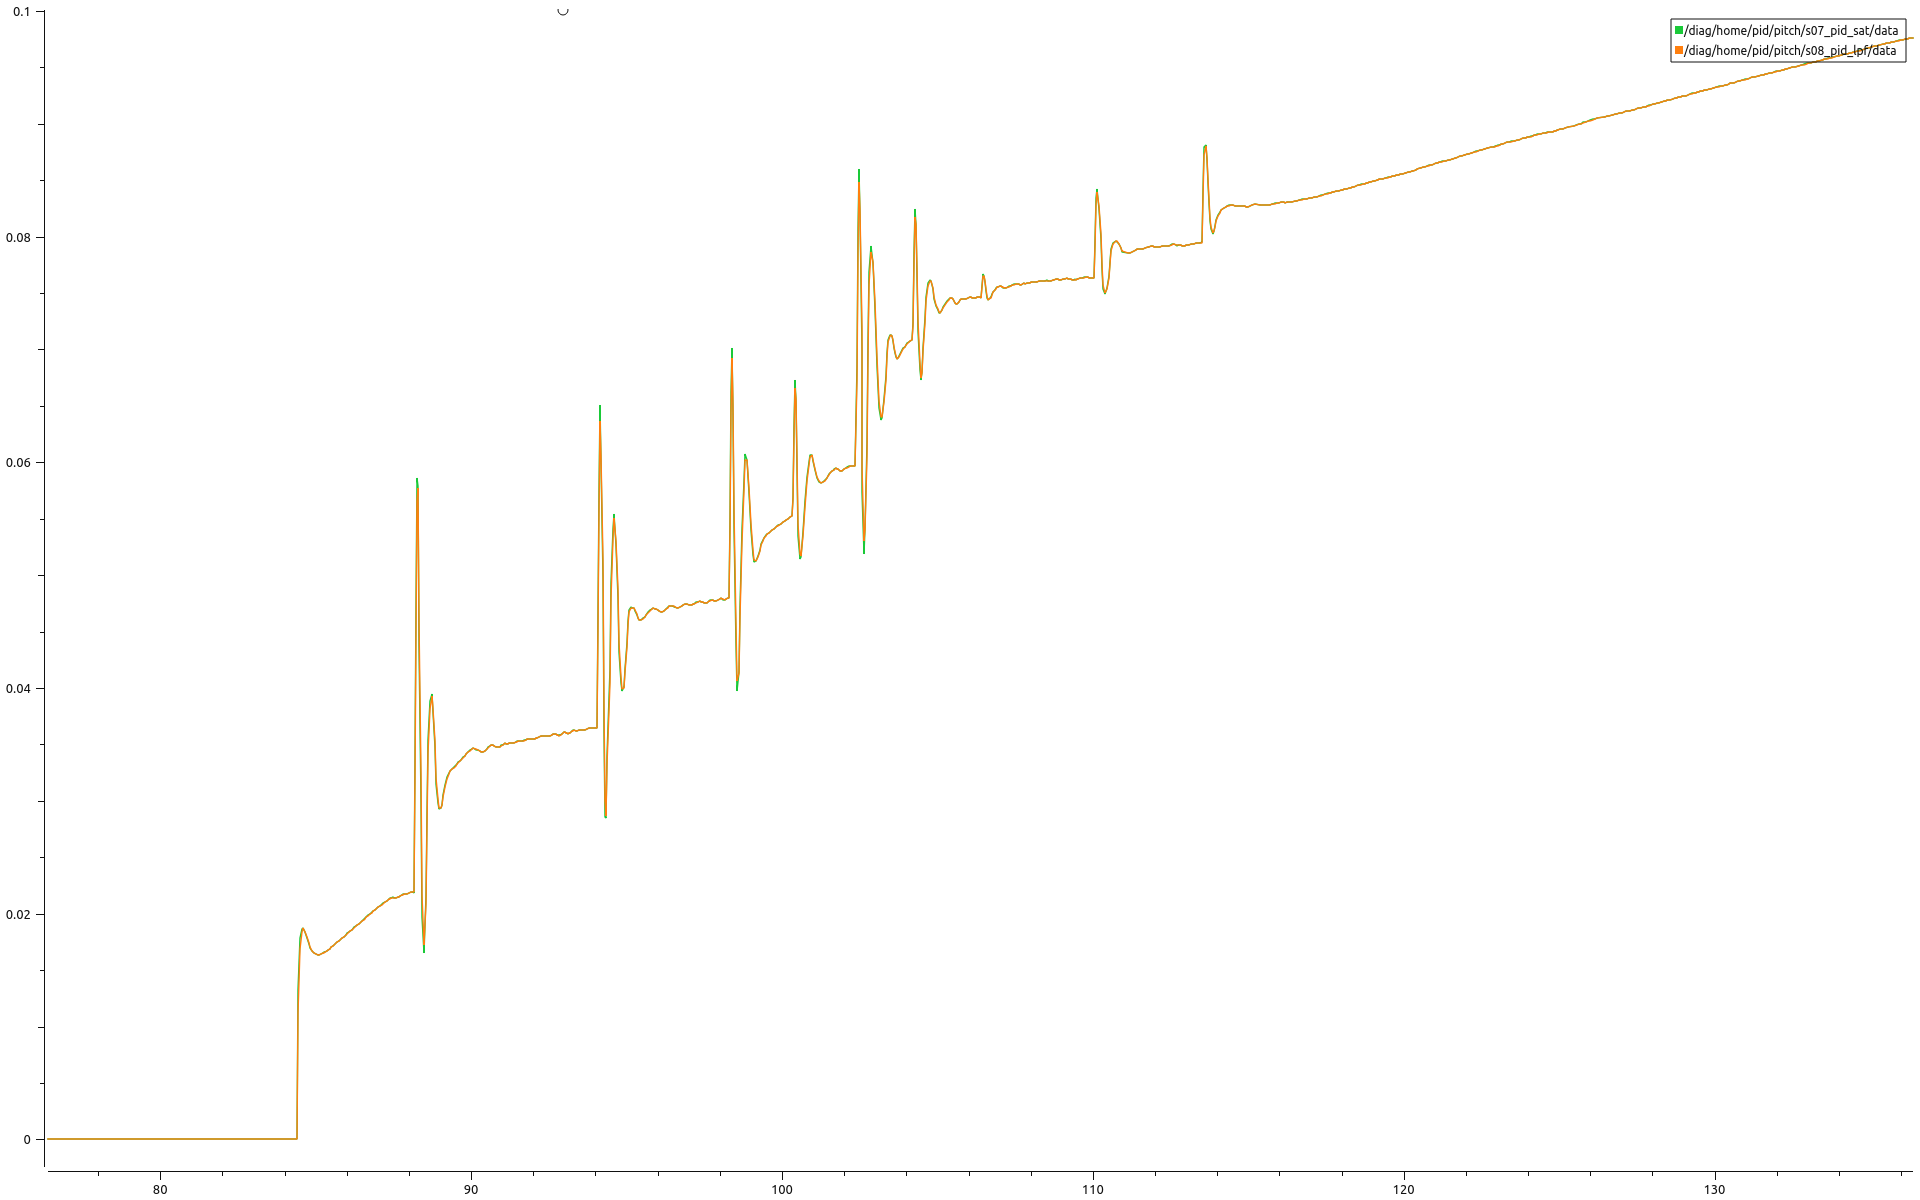
\includegraphics[width=\textwidth]{figures/imu_balance_homing_corr.png}
        \caption{PID and LPF output.}
        \label{fig:home_corr}
    \end{subfigure}

    \vspace{0.15cm}
    \begin{subfigure}[b]{0.44\columnwidth}
        \centering
        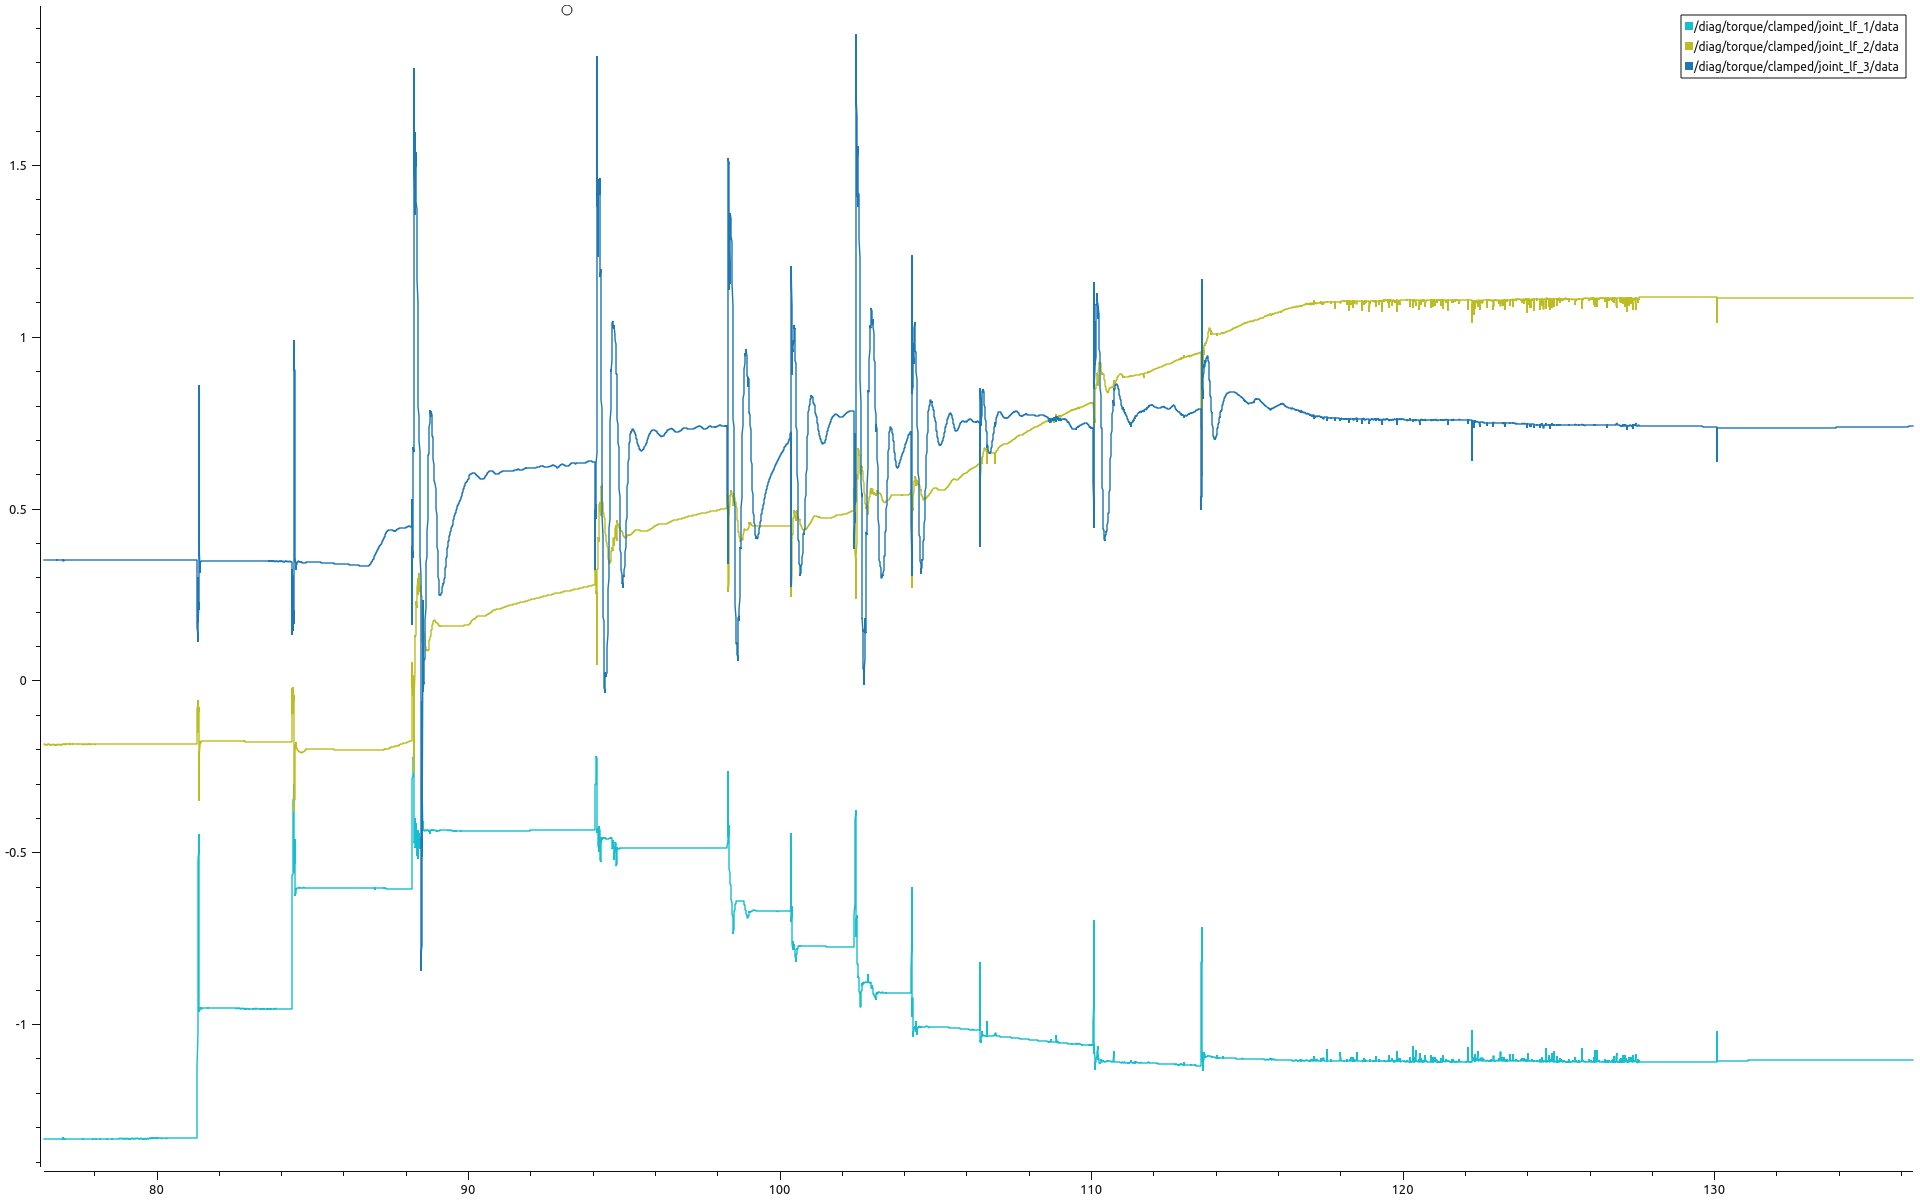
\includegraphics[width=\textwidth]{figures/imu_balance_homing_jointlf.png}
        \caption{Left front joint torques.}
        \label{fig:home_joint}
    \end{subfigure}

    \vspace{0.3cm}
    \caption{Home posture stabilization diagnostics.
    (a)~Pitch measurement and deadband filtered error.
    (b)~Saturated PID and lowpass filtered correction output.
    (c)~Resulting joint torque commands for the left front limb.}
    \label{fig:home_results}
\end{figure}

\subsection{Sinusoidal Platform Disturbance Response}

To quantify closed-loop disturbance rejection, the simulation
platform was driven by a $10^\circ$ amplitude, 30\,s period
sinusoidal tilt on both the roll and pitch axes independently.
The commanded tilt angle is published by the ramp-mover node on
\texttt{/diag/balance/disturbance/\{axis\}} and logged
simultaneously with the Home PID diagnostics on
\texttt{/diag/balance/home/\{axis\}/\{signal\}}.

Fig.~\ref{fig:pid_roll} shows the roll axis response. The IMU
filtered signal (\texttt{imu\_filtered}) tracks the commanded
disturbance with a slight lag introduced by the EMA pre-filter
($\alpha = 0.4$) and body inertia. The PID error signal
(\texttt{pid\_error}) oscillates in anti-phase: the controller
generates a restoring correction that partially compensates the
tilt. The deadzone band ($\pm 0.02$\,rad, shaded) visibly
suppresses the error during small-amplitude crossings, preventing
actuator chatter at steady state. The smoothed PID correction
output (\texttt{output\_smoothed}) presents a continuous,
low-noise signal suitable for direct joint-level actuation.

Fig.~\ref{fig:pid_pitch} presents the equivalent pitch axis
result. The pitch disturbance is phase-shifted by $90^\circ$
relative to roll (i.e.\ pitch lags roll by one quarter period),
reflecting the decoupled, independent sine wave applied by the
ramp-mover node. The qualitative behaviour is identical:
the filtered IMU response closely follows the commanded
disturbance, and the PID correction output is bounded and smooth,
confirming that the Home PID pipeline maintains stability under
simultaneous two-axis perturbations.

\begin{figure}[htbp]
    \centering
    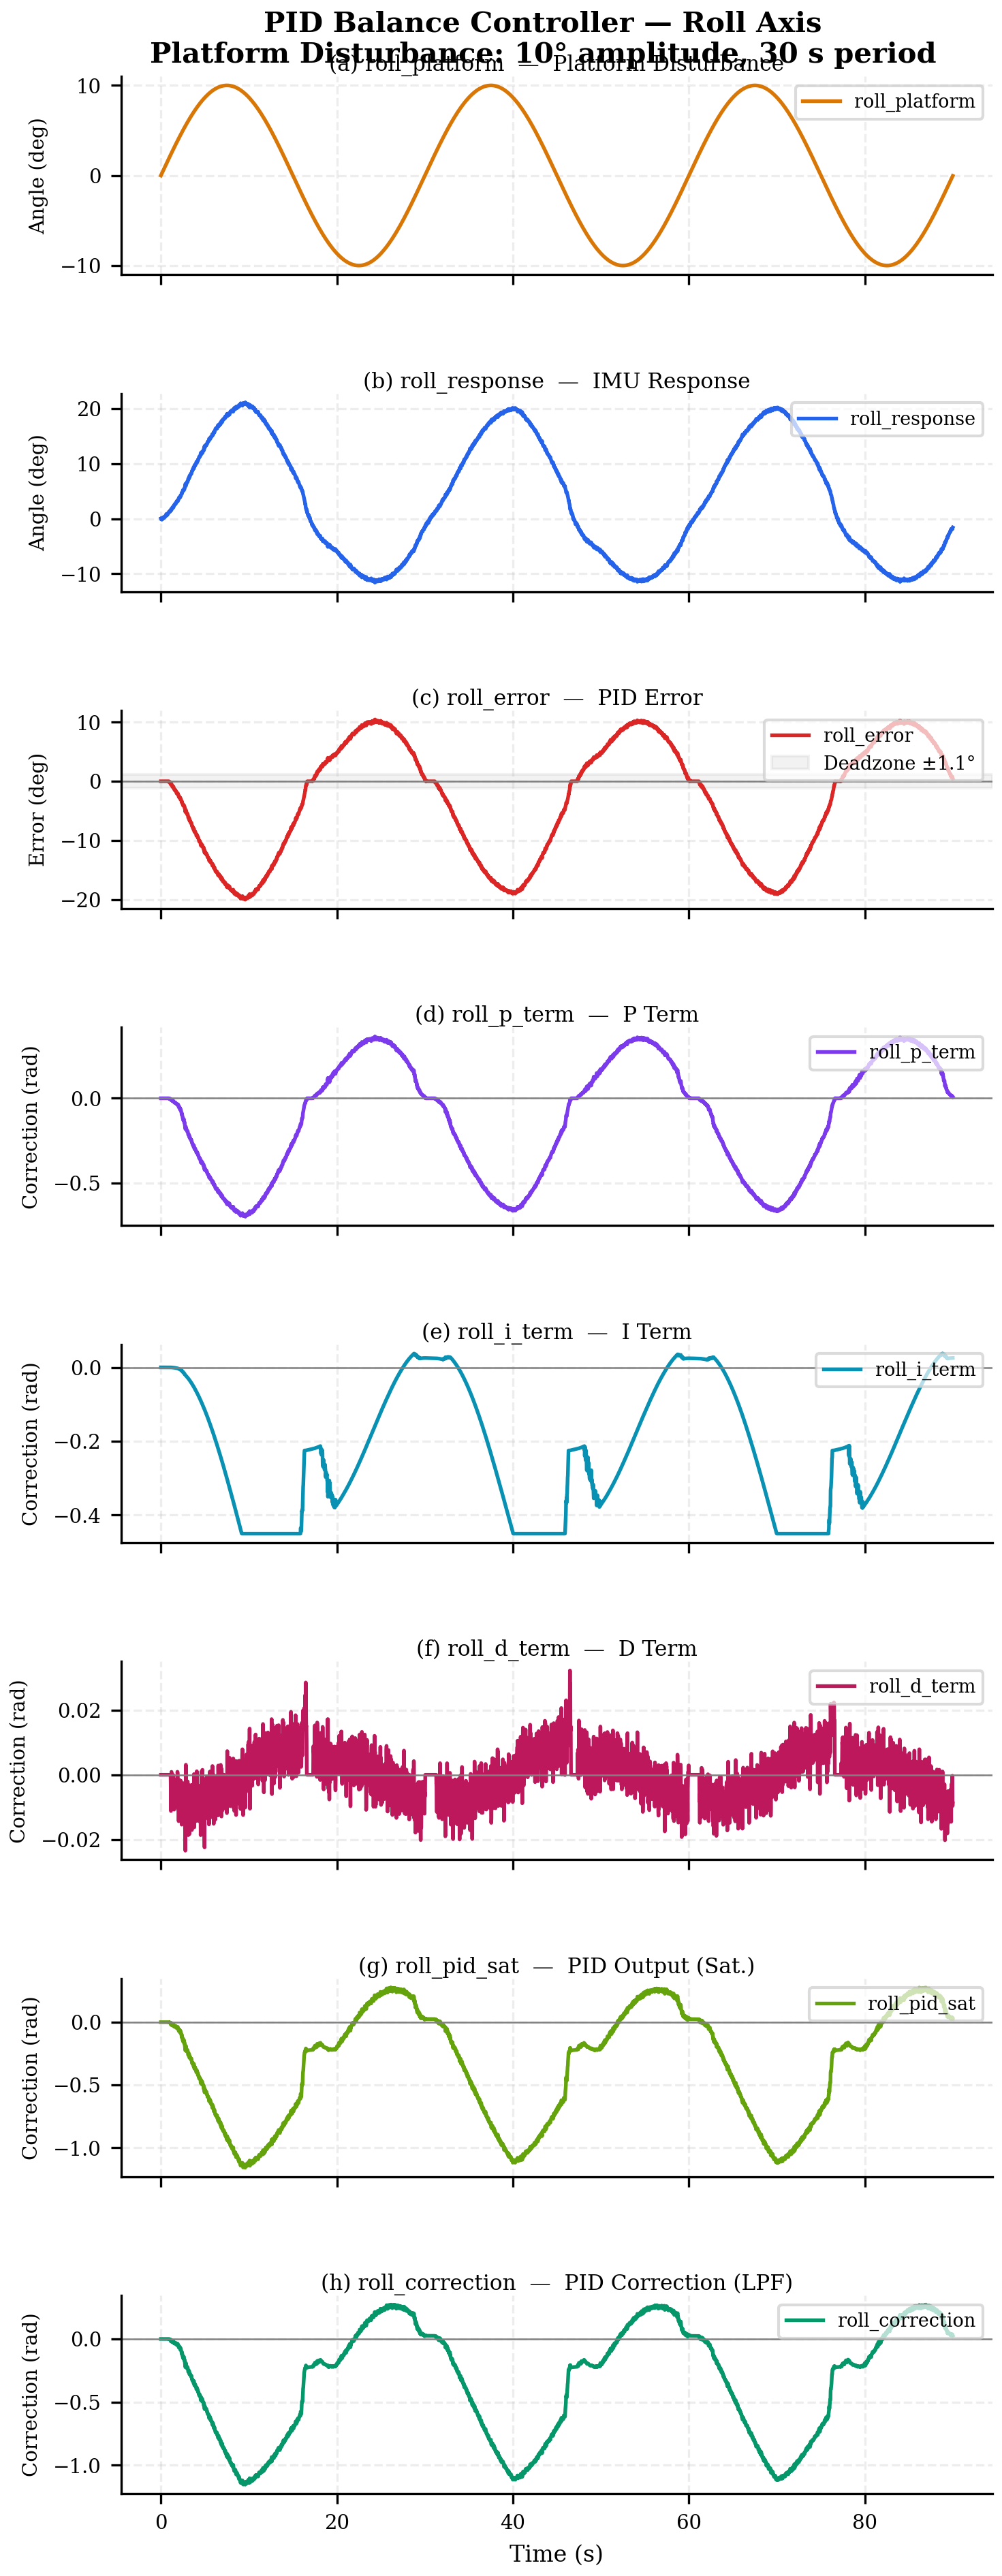
\includegraphics[width=\columnwidth]{figures/pid_balance_roll.png}
    \caption{Roll axis PID balance response under a sinusoidal
    platform disturbance ($A=10^\circ$, $T=30$\,s).
    (a)~Commanded ramp roll angle
    (\texttt{/diag/balance/disturbance/roll}).
    (b)~EMA-filtered IMU roll measurement
    (\texttt{/diag/balance/home/roll/imu\_filtered}).
    (c)~PID error after deadzone suppression
    (\texttt{/diag/balance/home/roll/pid\_error}).
    (d)~Final smoothed PID correction output
    (\texttt{/diag/balance/home/roll/output\_smoothed}).}
    \label{fig:pid_roll}
\end{figure}

\begin{figure}[htbp]
    \centering
    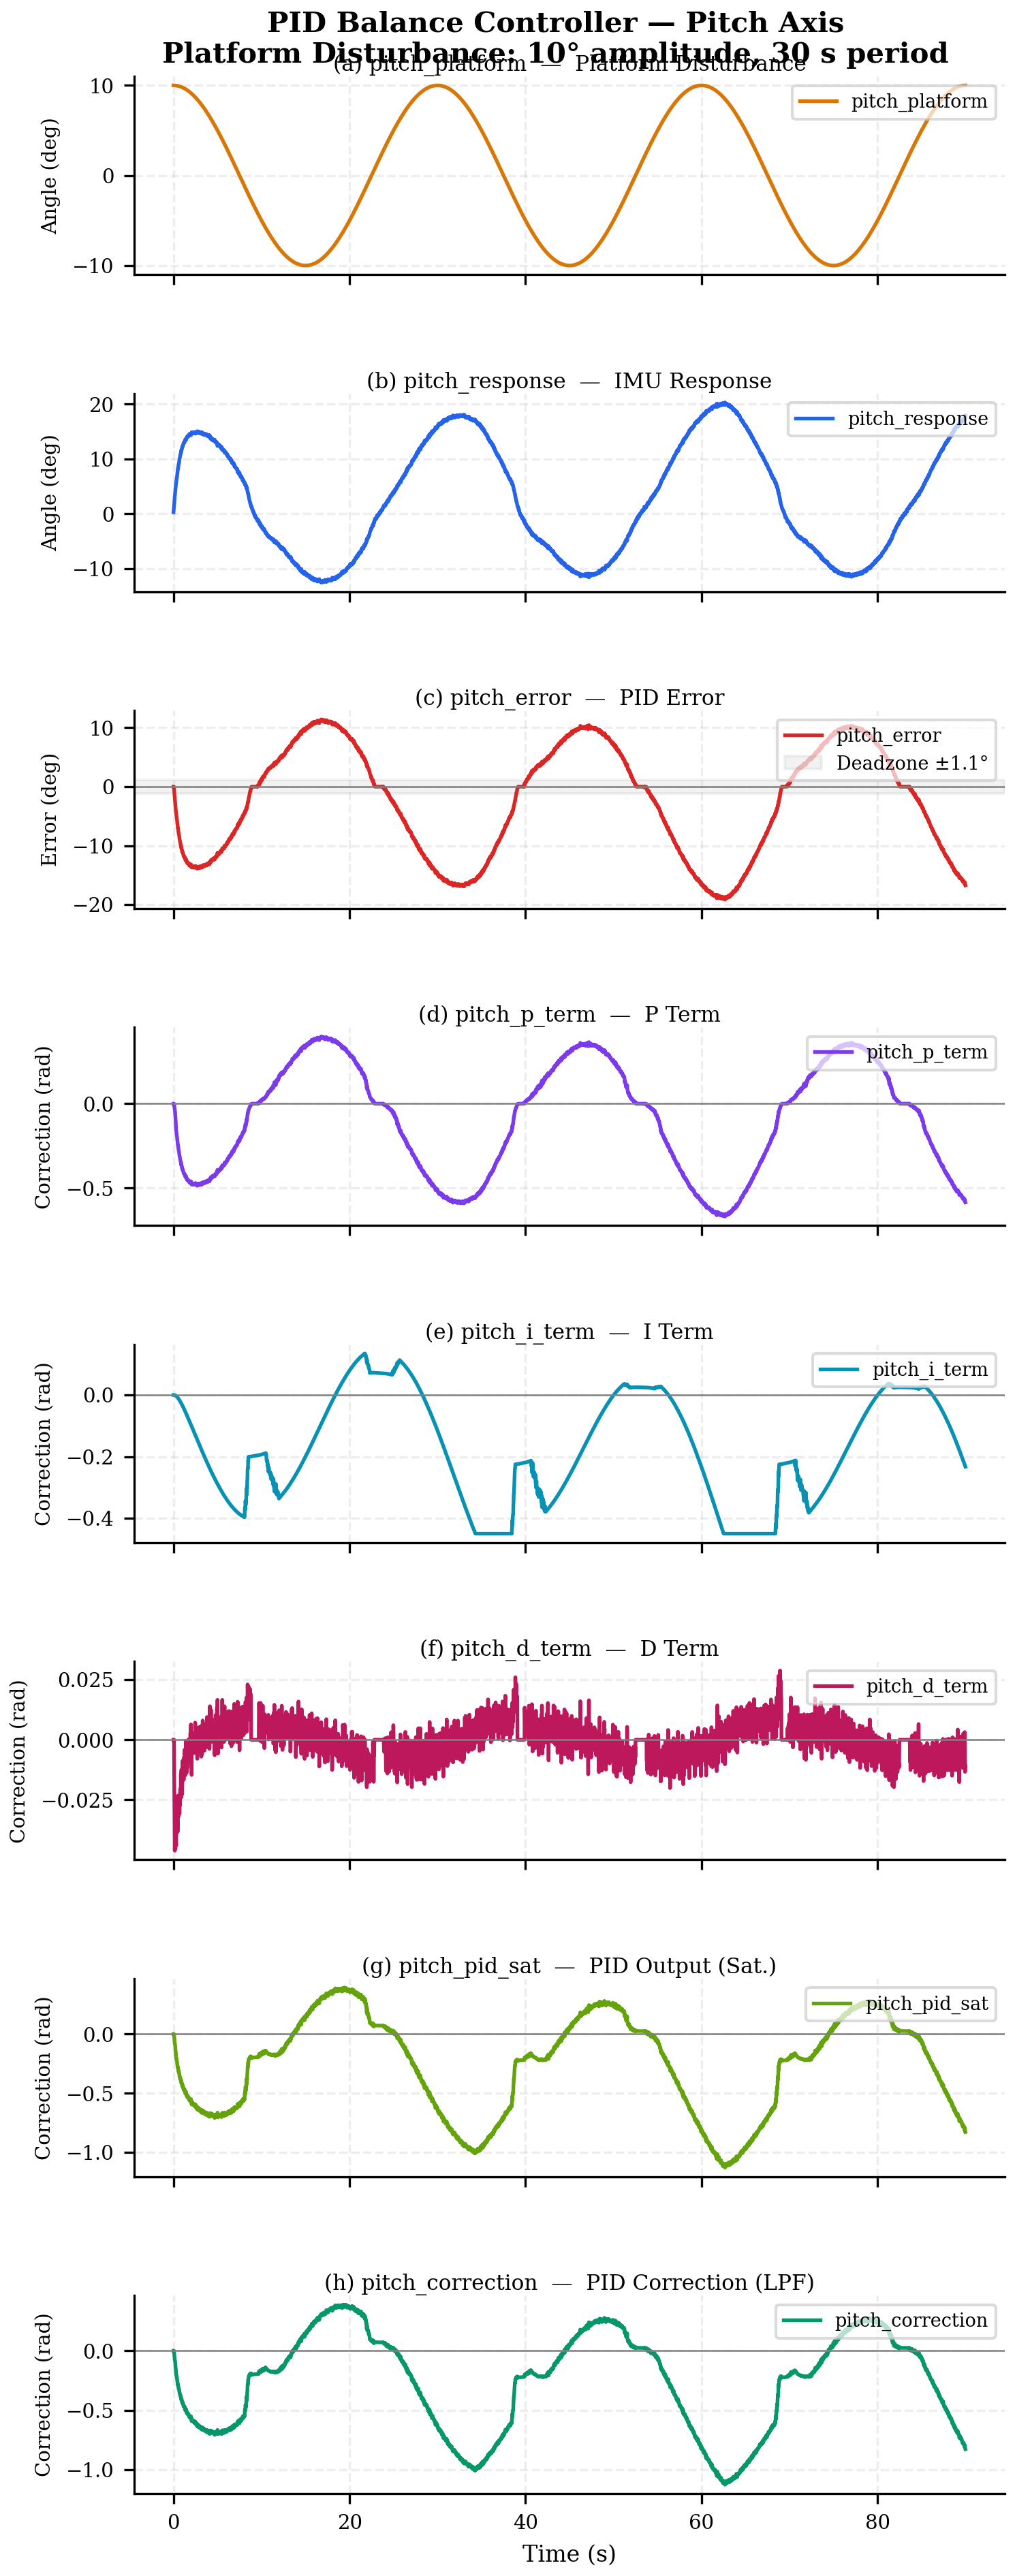
\includegraphics[width=\columnwidth]{figures/pid_balance_pitch.png}
    \caption{Pitch axis PID balance response under a sinusoidal
    platform disturbance ($A=10^\circ$, $T=30$\,s, phase offset
    $\varphi = 90^\circ$ relative to roll).
    (a)~Commanded ramp pitch angle
    (\texttt{/diag/balance/disturbance/pitch}).
    (b)~EMA-filtered IMU pitch measurement
    (\texttt{/diag/balance/home/pitch/imu\_filtered}).
    (c)~PID error after deadzone suppression
    (\texttt{/diag/balance/home/pitch/pid\_error}).
    (d)~Final smoothed PID correction output
    (\texttt{/diag/balance/home/pitch/output\_smoothed}).}
    \label{fig:pid_pitch}
\end{figure}

\subsection{Dynamic Trotting Gait Stabilization}

During active trotting locomotion, the adaptive PID controller
specific to the gait cycle maintains postural stability while the
quadruped executes cyclic quintic trajectories.
Fig.~\ref{fig:trot_results} presents the complete trotting mode
diagnostic dataset. The pitch axis measurement and error signals
(Fig.~\ref{fig:trot_error}) exhibit characteristic periodic
oscillations inherent to legged locomotion. The moving average
error signal successfully extracts the sustained tilt trend from
the cyclic gait artifacts, enabling the adaptive PID to distinguish
genuine disturbances from normal locomotion dynamics.
The corresponding PID correction output (Fig.~\ref{fig:trot_corr})
demonstrates the adaptive proportional gain responding to large
tilt events with elevated correction authority, while the lowpass
filtered output produces the smooth signal published to the gait
generator for stance phase rotational compensation. The resulting
joint torques (Fig.~\ref{fig:trot_joint}) display cyclic profiles
reflecting swing to stance phase transitions, with the stance phase
rotational compensation visible as high frequency modulation
in $\theta_3$.

\begin{figure}[htbp]
    \centering
    \begin{subfigure}[b]{0.44\columnwidth}
        \centering
        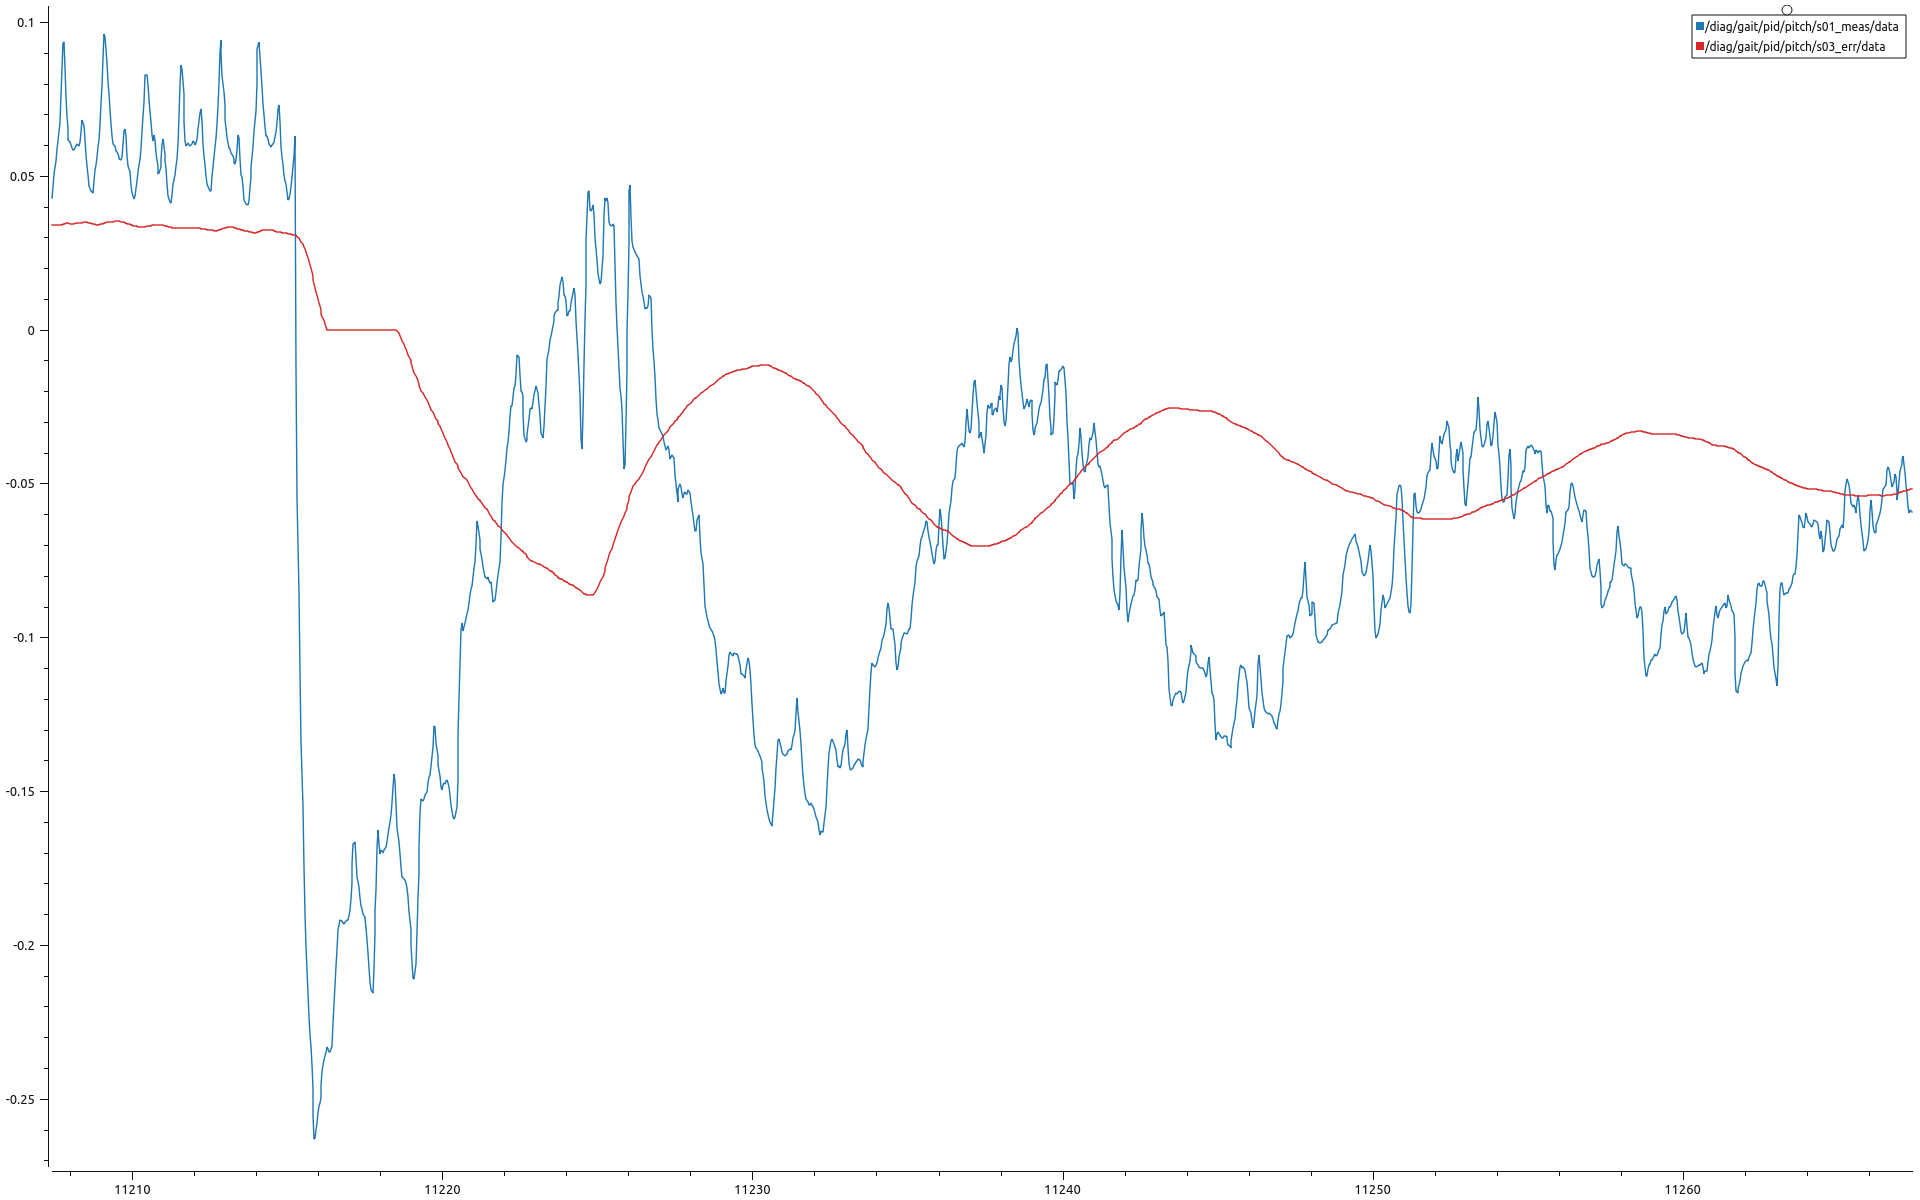
\includegraphics[width=\textwidth]{figures/imu_balance_trotting_error.png}
        \caption{Pitch and error.}
        \label{fig:trot_error}
    \end{subfigure}
    \hfill
    \begin{subfigure}[b]{0.44\columnwidth}
        \centering
        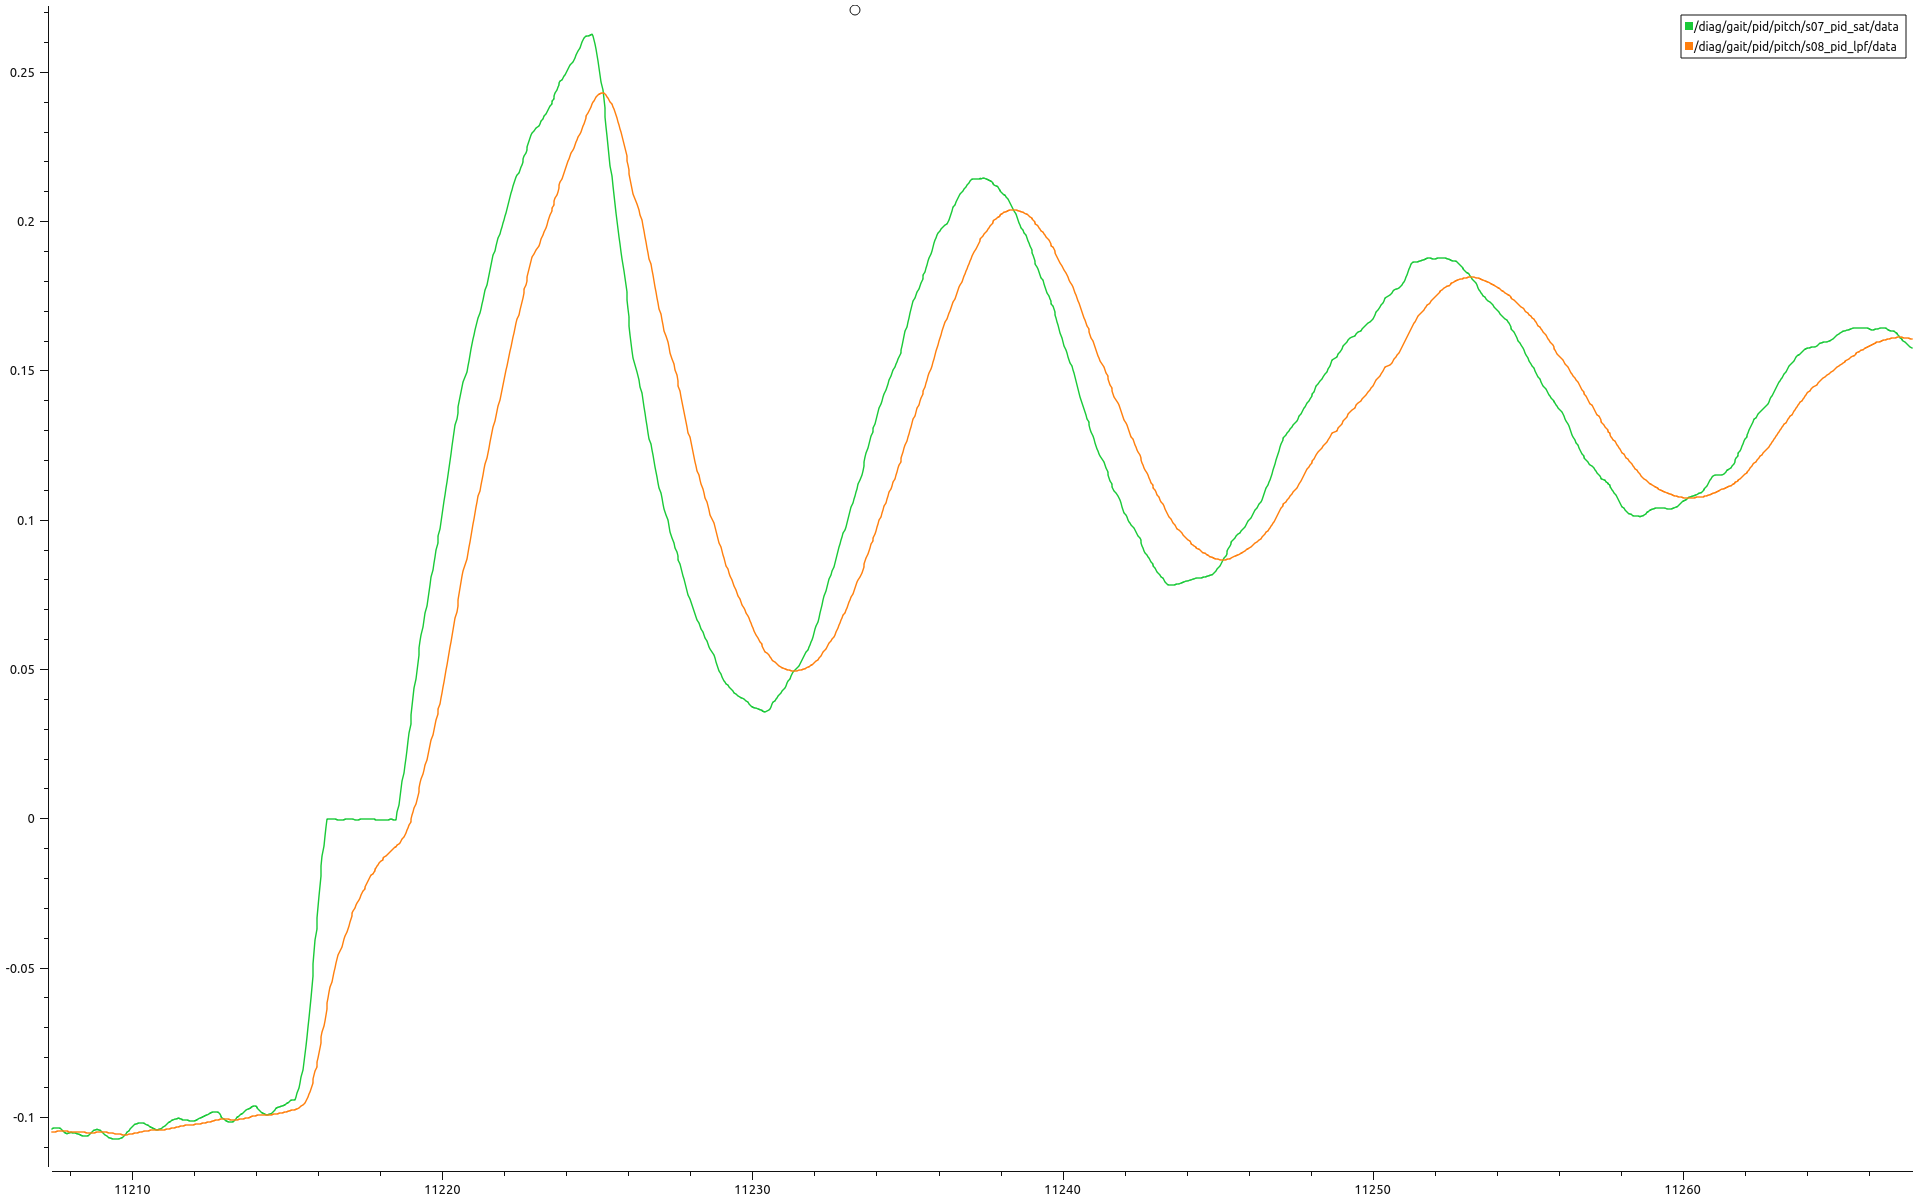
\includegraphics[width=\textwidth]{figures/imu_balance_trotting_corr.png}
        \caption{PID and LPF output.}
        \label{fig:trot_corr}
    \end{subfigure}

    \vspace{0.15cm}
    \begin{subfigure}[b]{0.44\columnwidth}
        \centering
        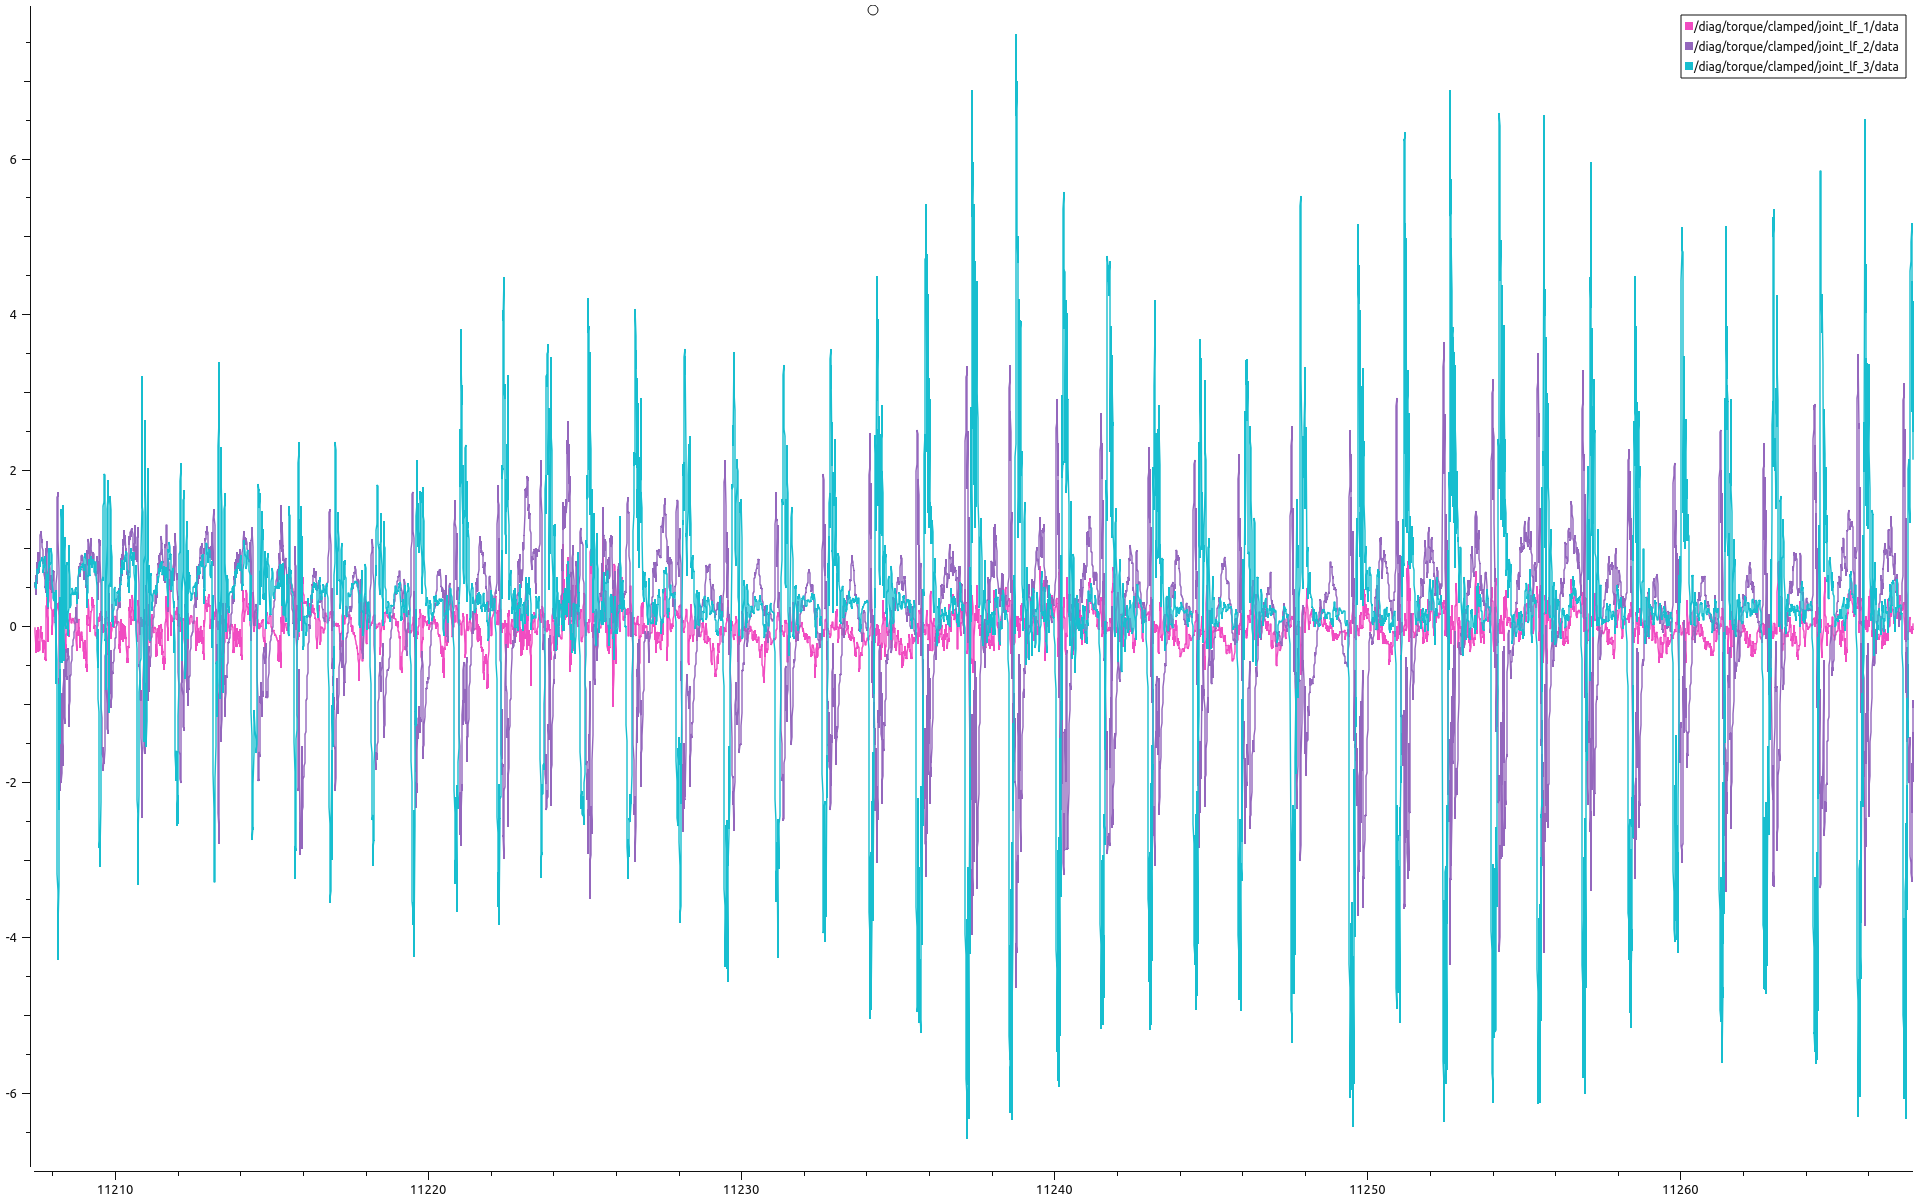
\includegraphics[width=\textwidth]{figures/imu_balance_trotting_jointlf.png}
        \caption{Left front joint torques.}
        \label{fig:trot_joint}
    \end{subfigure}

    \vspace{0.3cm}
    \caption{Dynamic trotting gait stabilization diagnostics.
    (a)~Pitch measurement and moving average error.
    (b)~Adaptive PID and lowpass filtered correction output.
    (c)~Resulting joint torque commands for the left front limb.}
    \label{fig:trot_results}
\end{figure}
